\documentclass[size36_42,landscape]{a0poster}
\usepackage{a0poster}
\usepackage{theorem,graphics,epsfig,amssymb,amsfonts,amsmath,multicol,multirow,hhline,wrapfig,times,float,url}
\usepackage{graphicx}
\usepackage[TABTOPCAP]{subfigure}
\usepackage{algorithm}
\usepackage{algorithmic}
\usepackage{fancybox}
\usepackage{shadow}
%\usepackage{pstricks,pst-node}
%\usepackage{wasysym}
\usepackage[absolute]{textpos}
\usepackage{color}

\usepackage{natbib}


\usepackage{sidecap}
\usepackage{anyfontsize}
\usepackage{setspace,nicefrac}

% \usepackage{graphicx}

\usepackage{array}% http://ctan.org/pkg/array


\newcommand{\COMMENTEQ}[2][3em]{%
  \leavevmode\hfill\makebox[#1][l]{//~#2}}


\usepackage{tikz,xifthen}
\def\tikzmark#1{\tikz[remember picture,overlay]\coordinate(#1);}
\usetikzlibrary{arrows}

\tikzstyle{every picture}+=[remember picture]

\tikzstyle{notebox}=[draw=none,anchor=base,inner sep=0,outer sep=0]

% \usepackage{lipsum}
% \usepackage{twoopt}
% \usepackage{letltxmacro}


%\usepackage[noamsthm]{beamerarticle}
%\mode<presentation>{\usetheme{Madrid}}
%\definecolor{darkblue}{rgb}{0.1,0.1,0.5}
%\definecolor{lightblue}{rgb}{.68,.85,.9}
%\definecolor{brown}{cmyk}{0,0.81,1,0.60}
%\definecolor{problem}{rgb}{0.9,0.8,0.8}
%\definecolor{purple}{rgb}{0.4,0,0.4}
\def\CBOX#1{\colorbox{yellow}{#1}}
\def\CBOXG#1{\colorbox{green}{#1}}
%\pagestyle{empty}
\setcounter{secnumdepth}{0}
\setlength{\columnsep}{1cm}
\setlength{\fboxsep}{0pt}
\setlength{\fboxrule}{5pt}
%listicon
\usepackage{pifont}
% \newcommandtwoopt{\xyz}[3][Def1][Def2]{Something with #1, #2 and #3}

\newenvironment{coldinglist}[2]	    {
\begin{list}
  {\textcolor{#2}{\ding{#1}}}{
\setlength{\parskip}{0pt}
\setlength{\itemsep}{0pt}
\setlength{\parsep}{0pt}
}
	}
	{\end{list}}
\floatstyle{ruled}
%\newcommand(\HR)
\def\ba{{\bf a}}
\def\bb{{\bf b}}
\def\bc{{\bf c}}
\def\bd{{\bf d}}
\def\be{{\bf e}}
\def\bp{{\bf p}}
\def\bq{{\bf q}}
\def\bw{{\bf w}}
\def\bx{{\bf x}}
\def\by{{\bf y}}
\def\bz{{\bf z}}
\def\bu{{\bf u}}
\def\bv{{\bf v}}
\def\bk{{\bf k}}
\def\bff{{\bf f}}
\def\bzero{{\bf 0}}
\def\bone{{\bf 1}}
\def\b0{{\bf 0}}
\def\rij{r_{ij}}
\def\bomega{\boldsymbol \omega}
\def\bbeta{{\boldsymbol\beta}}
\def\beps{{\boldsymbol \epsilon}}
\def\diag{\mbox{\sf diag}}
\def\Zsym{\overline{Z}}
\def\calC{\mathcal{C}}
\def\calB{\mathcal{B}}
\def\calU{\mathcal{U}}
\def\calZ{\mathcal{Z}}
\def\tr{\mbox{tr}}
\def\imagetop#1{\vtop{\null\hbox{#1}}}
\renewcommand{\thesubfigure}{}


\definecolor{darkpastelgreen}{rgb}{0.01, 0.75, 0.24}
\newcommand{\paragraphHeader}[1]{\vspace{1cm}\par{\LARGE\bf\color{darkpastelgreen} \it{\underline{\hspace{.5em}#1\hspace{.5em}}}}\par\vspace{1cm}}

\DeclareMathOperator*{\argmax}{\arg\max}
\DeclareMathOperator*{\argmin}{\arg\min}


\begin{document}

%%%%%%%%%%%%%%%%%%%%%%%%%%%%%%%%%%%%
\title{Active Search and Bandits on Graphs Using Sigma-Optimality}
\author{Yifei Ma* and Tzu-Kuo Huang** and Jeff Schneider*}
\address{*Auton Lab, School of Computer Science, Carnegie Mellon University.  **Microsoft Research}
\email{yifeim@cs.cmu.edu, tkhuang@microsoft.com, schneide@cs.cmu.edu}
\makeheader
%%%%%%%%%%%%%%%%%%%%%%%%%%%%%%%%%%%%



\begin{multicols}{3}
\fontsize{36pt}{43pt}\selectfont
\setlength{\columnsep}{1.5cm}
\setlength{\columnseprule}{0.3pt}


%%%%%%%%%%%%%%%%%%%%%%%%%%%%%%%%%%%%
\paragraphHeader{Problem Setup}
%%%%%%%%%%%%%%%%%%%%%%%%%%%%%%%%%%%%

\begin{coldinglist}{113}{blue}
\item Given an undirected graph: edges given, nodes unlabeled
\item Search for (i.e., query) all positive nodes
\item Feedback provided as each node is queried
\item Use similarity as hint
\end{coldinglist}

%%%%%%%%%%%%%%%%%%

\usetikzlibrary{positioning}
\tikzset{
    position/.style args={#1:#2 from #3}{
        at=(#3.center), anchor=center, shift=(#1:#2)
    },
    nil/.style = {draw,circle,
   minimum size=0.7*\nodeDist, node distance=0pt,
    inner sep=0pt,
    outer sep=0,
    ultra thick,
   },
    target/.style = {nil,draw=none, fill=white, text=darkpastelgreen},
   seed/.style = {nil, draw=black, minimum size=0.7*\nodeDist, line width=2mm,
   },
   ucb/.style = {seed, draw=blue,   },
   sopt/.style = {seed, draw=red,   },
}


\newcommand{\nodeDist}{3cm}

\newcommand{\toyPlot}{
  \node [nil] (n1) {};
  \node [nil, position=20:{\nodeDist} from n1] (n2) {};
  \node [nil, position=45:{\nodeDist} from n2] (n3) {};
  \node [nil, position=-90:{1.5*\nodeDist} from n3] (n4) {};
  \node [nil, position=0:{1.5*\nodeDist} from n2] (n5) {};
  \node [nil, position=-60:{\nodeDist} from n5] (n6) {};
  \node [nil, position=-80:{\nodeDist} from n6] (n7) {};
  \node [nil, position=-60:{\nodeDist} from n7] (n8) {};
  \node [nil, position=0:{2*\nodeDist} from n8] (n9) {};
  \node [nil, position=10:{\nodeDist} from n8] (n10) {};
  \node [nil, position=60:{\nodeDist} from n8] (n11) {};
  \node [nil, position=60:{\nodeDist} from n11] (n12) {};
  \node [nil, position=60:{\nodeDist} from n12] (n13) {};   \node [nil, position=40:{\nodeDist} from n13] (n14) {};   \node [nil, position=-40:{\nodeDist} from n14] (n15) {};   \node [nil, position=20:{\nodeDist} from n14] (n16) {};
  \node [nil, position=-20:{\nodeDist} from n16] (n17) {};

  \draw (n1) -- (n2) -- (n3) -- (n5) -- (n4) -- (n2);
  \draw (n2) -- (n5);
  \draw (n3) -- (n4);
  \draw (n3) -- (n5) -- (n6) -- (n7);
  \draw (n7) -- (n8) -- (n10) -- (n12) -- (n7);
  \draw (n7) -- (n11) -- (n10);
  \draw (n8) -- (n11) -- (n12);
  \draw (n9) -- (n10);
  \draw (n12) -- (n13) -- (n14) -- (n15) -- (n16) -- (n14);
  \draw (n16) -- (n17);
}

%%%%%%%%%%%%%%%%%%

\newcommand{\toytargets}{2,3,5,7,8,11,14,15}

\begin{center}
\vspace{-.5em}
\begin{tikzpicture}
  \toyPlot
  % seed nodes
  \foreach \x in {1,...,17}{
    \node[draw=none] at (n\x) {?};
  }
  \foreach \x in {2,3,4,5}{
    \node[text=red, fill=white, draw=none] at (n\x) {$\times$};
    % \node[draw=none, text=red] at (n\x){$\times$};
    \foreach \y in \toytargets {
        \ifthenelse{\x = \y}{
            \node[target] at (n\x) {$\checkmark$};
        }{}
    }
    \node[seed] at (n\x){};
  }
  % selections
  \node [ucb] at (n17) {};
  \node [sopt] at (n11) {};
  \node [nil, draw=none, position=0:{4*\nodeDist} from n11] (textcenter) {};
  \node [draw=none, anchor=base] (text) at (textcenter) {Which node to query next?};
  \path[-triangle 90, draw=red, ultra thick] (n11) edge [out=0, in=-90] (text);
  \path[-triangle 90, draw=blue, ultra thick] (n17) edge [out=-45, in=90] (text);
  % node id
%   \foreach \x in {1,...,17}
%   {
%     \node [draw=none, below right=.1\nodeDist of n\x.center, minimum size=5pt] {\textbf{$\mathbf{\x}$}};
%   }
  
\end{tikzpicture}
\vspace{-3em}
\end{center}


%%%%%%%%%%%%%%%%%%

%%%%%%%%%%%%%%%%%%%%%%%%%%%%%%%%%%%%
\paragraphHeader{Related Work}
%%%%%%%%%%%%%%%%%%%%%%%%%%%%%%%%%%%%
\begin{coldinglist}{112}{blue}
\item Query strategy needs to balance:
\begin{coldinglist}{123}{blue}
\item \tikz[baseline,remember picture]{\node[notebox,fill=blue!20,anchor=base] {Exploitation:};} query nodes that are mostly likely targets
\item \tikz[baseline,remember picture]{\node[notebox,fill=green!20,anchor=base] {Exploration:};} get the most information about label distribution
\end{coldinglist}

\item GP-UCB [Srinivas et al. 2010; Gotovos et al. 2013] 
\begin{coldinglist}{123}{blue}
\item Bayes assumption $f \sim \mathcal{GP}(\mu, c) $



 \item Decision rule $v_{t+1}\leftarrow \argmax_v
 \tikz[baseline,remember picture]{\node[fill=blue!20,anchor=base] (mut) {$ \mu_t(v)$};}
 +
 \tikz[baseline,remember picture]{\node[fill=red!20, circle, anchor=base] (aat) {$ \alpha_t$};}
 \tikz[baseline,remember picture]{\node[fill=green!20,anchor=base] (sigmat) {$ \sigma_t(v)$};}
 $.

 
\hspace{1.5em}
\tikz[baseline]{\node[notebox,fill=blue!20] (mutt) {Exploitation (post mean)};}, \tikz[baseline]{\node[notebox,fill=red!20] (aatt) {Tradeoff};}, \tikz[baseline]{\node[notebox,fill=green!20] (sigmatt) {Exploration (post std)};}

\item In practice, often explore boundaries first ...
% 
    % \item Current literature [Krause et al., 2008; Srinivas et al., 2010; Gotovos et al., 2013; Valko et al., 2014] 
    % explores by $\argmax_v \sigma_t(v)$; often explores boundaries first; worse in high dimensions
    %$\Sigma$-optimality from survey risk reduction
    \begin{center}
    {\footnotesize [Krause et al. 2008]}\hspace{-1em}
    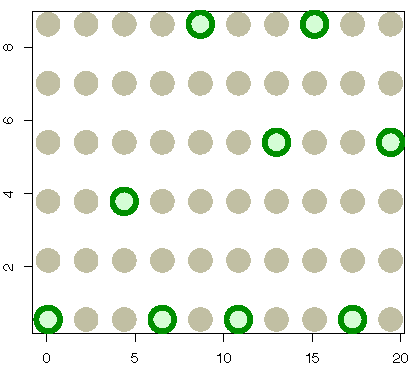
\includegraphics[width=.27\linewidth]{krause_boundary.pdf}
    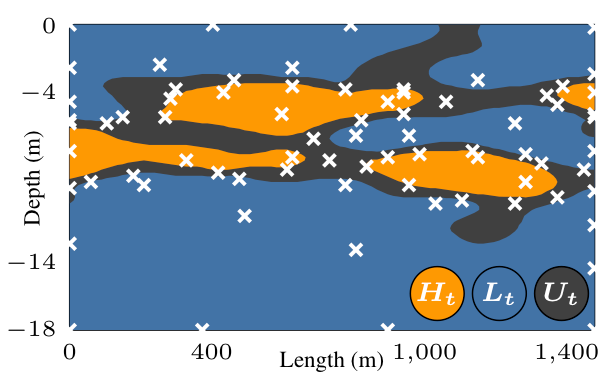
\includegraphics[width=.4\linewidth]{pond_boundary.pdf}
    \hspace{-1em}
    {\footnotesize [Gotovos et al. 2013]}
    \end{center}
    
\end{coldinglist}

\begin{tikzpicture}[overlay]
\draw [-triangle 90,draw=red,ultra thick] (mut) -- (mutt);
\draw [-triangle 90,draw=red,ultra thick] (aat) -- (aatt);
\draw [-triangle 90,draw=red,ultra thick] (sigmat) -- (sigmatt);
\end{tikzpicture}
\vspace{-1.5em}

%%%%%%%%%%%%%%
\item Spectral-UCB [Valko et al. 2014]
\begin{coldinglist}{123}{blue}
\item Graph kernel from regularized Laplacian, $c(v,v')=\mathbf{1}_{v}^\top\mathcal{\tilde{L}}^{-1}\mathbf{1}_{v'}$
\item Algorithm unchanged;
theoretical guarantees improved
\item Still explores boundaries first ...
\end{coldinglist}
\end{coldinglist}

%%%%%%%%%%%%%%%%%%%%%%%%%%%%%%%%%%%%
\paragraphHeader{Main Contributions}
%%%%%%%%%%%%%%%%%%%%%%%%%%%%%%%%%%%%

\begin{center}
\begin{tikzpicture}[scale=0.6, transform shape]
  \toyPlot
  % ucb selection, alpha=.3, sigma_n^2=1, omega_0=0.01, mu_0=0. 
  % [~, S] = AS_UCB(A, .3, label_toy_bin', struct('start_point',7,'num_evaluations',5,'obs_sigma',1))
  \foreach \x in {7,17,1,9,8}{ %11 %{7,17,1,9,15,13} {
    \node[draw=none, text=red] at (n\x){$\times$};
    \foreach \y in \toytargets{ %{7,8,11,15,16}{
       \ifthenelse{\x = \y}{\node[target] at (n\x){$\checkmark$};}{}
  }
  \node[ucb] at (n\x){};
  }
\end{tikzpicture}
% 
\begin{tikzpicture}[scale=0.6, transform shape]
  \toyPlot
   % sopt selection, alpha=.3, sigma_n^2=1, omega_0=0.01, mu_0=0
   % [~, S] = AS_MI_sopt(A,.3,label_toy_bin',struct('start_point',7,'num_evaluations',5,'obs_sigma',1))
  \foreach \x in {7,14,2,10,5} %16 %{7,13,5,2,4,8}%{7,14,2,10,16,5}
  {
  \node[draw=none, text=red] at (n\x){$\times$};
   \foreach \y in \toytargets{ %{7,8,11,15,16}{
     \ifthenelse{\x = \y}{\node[target] at (n\x){$\checkmark$};}{}
  }
  \node[sopt] at (n\x) {};
  }
\end{tikzpicture}
\end{center}
\begin{center}
Choices in previous work \hspace{3em} Choices by our algorithm
\end{center}

%%%%%%%%%%%%%%%%%%%%%%%%%%%

\begin{coldinglist}{112}{blue}
\item New \tikz[baseline]{\node[notebox,fill=green!20] {exploration term};}: favor cluster centers over boundaries
\begin{coldinglist}{123}{blue}
    \item Measured by improvement of $\Sigma$-optimality [Ma et al. 2013]
    % \item Use $\Sigma$-optimality [Ma et al. 2013]
\end{coldinglist}
\item High probability regret bounds; compare with
\begin{coldinglist}{123}{blue}
    \item{} [Srinivas et al. 2010; Valko et al. 2014; Contal et al. 2014]
\end{coldinglist}
\item Empirical results
\end{coldinglist}



% \tikzmark{D}
% \begin{flushright}
% \vspace{-2em}
% 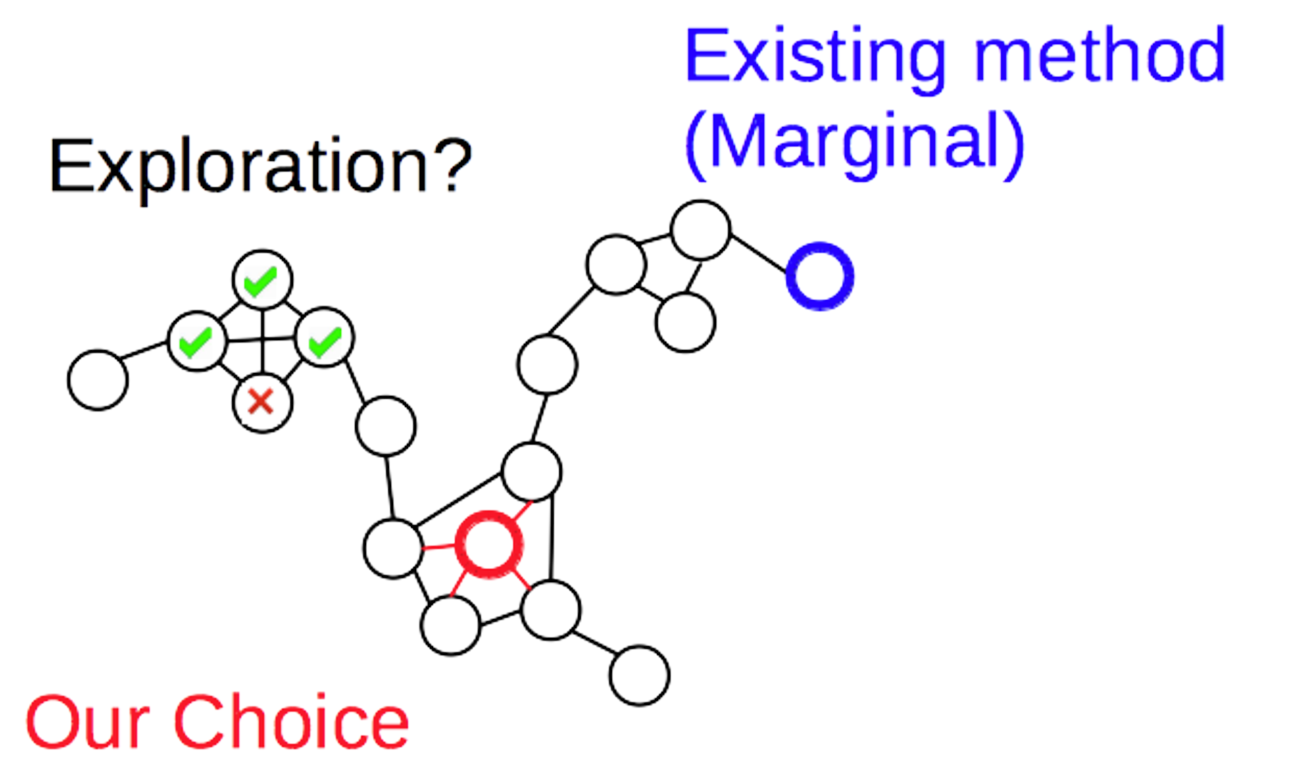
\includegraphics[width=.55\linewidth]{toy_plot.pdf}\hspace{-1em} 
% \vspace{-4em}
% \end{flushright}

% \begin{tikzpicture}[remember picture, overlay]
%   \node[anchor=north west, text width=.42\linewidth, inner sep=0,outer sep=0] at (D) {High intrinsic dimension; naive exploration (current) tends to select leaf nodes.};
% \end{tikzpicture}



   

\vfill
\columnbreak

%%%%%%%%%%%%%%%%%%%%%%%%%%%%%%%%%%%%
\paragraphHeader{Bayes Model (GRF) [Zhu et al. 2003]}
%%%%%%%%%%%%%%%%%%%%%%%%%%%%%%%%%%%%
% \newcommand{\bff}{\mathbf{f}}
\newcommand{\bmu}{\boldsymbol{\mu}}
\newcommand{\bC}{\mathbf{C}}
\newcommand{\bA}{\mathbf{A}}
\newcommand{\bD}{\mathbf{D}}
\newcommand{\cLap}{\boldsymbol{\mathcal{L}}}
\newcommand{\bH}{\mathbf{H}}
\newcommand{\bI}{\mathbf{I}}


\newcommand{\highlight}[2][yellow]{\mathchoice%
  {\colorbox{#1}{$\displaystyle#2$}}%
  {\colorbox{#1}{$\textstyle#2$}}%
  {\colorbox{#1}{$\scriptstyle#2$}}%
  {\colorbox{#1}{$\scriptscriptstyle#2$}}}%


% Gaussian random fields (GRF) [Zhu et al. 2008]

\begin{coldinglist}{113}{blue}
\item Every node $v_i$ has value $f(v_i)$; GRF prior in vector form $\bff$,
% 
% \item If select $v_t$, feedback $y(v_t) = f(v_t) + \epsilon,$ where $\epsilon\sim\mathcal{N}(0,\sigma_n^2)$
% 
% \item Assume Gaussian random field prior (positive adjacency $\bA$)
\begin{equation}
    \highlight{ \color{red} 
\bff \sim \mathcal{N}\Bigl( 
    		 \color{red} \bmu_0 } = \mu_0\cdot\bone, 
    		\highlight{ \phantom{\Bigl(} \color{red} \bC_0  } =\mathcal{\tilde{L}}^{-1} = \bigl(\bD - \bA + \omega_0 \bI\bigr)^{-1}
    	\Bigr), 
    	\label{eq:prior}
\end{equation}
\begin{center}\scalebox{0.8}{$ \displaystyle
\Leftrightarrow \quad
    \log 
    	p_0(\bff) 
    	 \simeq
    		-\sum_{i=1}^N\sum_{j=1}^N \frac{A_{ij}(f_i-f_j)^2}{2} -   \sum_{j=1}^N  \frac{\omega_0 (f_j-\mu_0)^2}{2}
$}
\end{center}
    where $\mu_0$, $\omega_0$ are hyper-parameters, $\bD$ degree diagonal matrix.
    Define usual  $C(v,v') = \rho(v,v')\sigma(v)\sigma(v')$.
    
    
\item Objective: cumulative reward in $T$ rounds, $\highlight{\color{red} \sum_{t=1}^T f_{v_t} }$, by active search with noisy feedback $y(v_t) = f(v_t) + \epsilon_t,$  $\epsilon_t\stackrel{iid}{\sim}\mathcal{N}(0,\sigma_n^2)$

\end{coldinglist}

%%%%%%%%%%%%%%%%%%%%%%%%%%%%%%%%%%%%
% \vfill
% \columnbreak
%%%%%%%%%%%%%%%%%%%%%%%%%%%%%%%%%%%%


%%%%%%%%%%%%%%%%%%%%%%%%%%%%%%%%%%%%
\paragraphHeader{Our Methods}
%%%%%%%%%%%%%%%%%%%%%%%%%%%%%%%%%%%%


\begin{center}
\vspace{-.4em}
\begin{minipage}{.9\linewidth}
\begin{algorithm}[H]
    \Large
	\caption{\Large \textsc{gp-sopt} and its variants}
% 	\label{alg:main}
	\begin{algorithmic}
  	\STATE \textbf{input} $\mu_0$, $\bA$, $\omega_0$, $\sigma_n$, $\alpha_t$, $T$;
  	if warm start, $\{v_\tau,y(v_\tau)\}_{\tau=1}^{t_0}$
	\STATE Obtain initial $\mathcal{N}(\bmu_{0},\bC_{0})$ \COMMENTEQ{\eqref{eq:prior}}
	\FOR{$t = t_0, \ldots, T-1,$}
 	\STATE Update to conjugate posterior $\mathcal{N}(\bmu_t, \bC_t)$ 
%  	\COMMENTEQ{\eqref{eq:prior}}
%  	\COMMENTEQ{\eqref{eq:post_prec}}
% 	\STATE Compute exploration $s_t(v)$  
% 	\STATE \CBOX{Select $\displaystyle v_{t+1} \leftarrow \argmax_{v \in V \setminus S_t} $\CBOX{$\mu_{t}(v)$}$ + \alpha_{t} s_{t}(v)$} \hfill \makebox[5em][r]{// (\ref{eq:sopt.orig}, \ref{eq:sopt.tt}, or \ref{eq:sopt.topk})}
% % \COMMENTEQ{\eqref{eq:selection}}
\STATE \CBOX{$\displaystyle v_{t+1}\leftarrow \argmax_{v\in V\setminus S_t}
 \tikz[baseline,remember picture]{\node[fill=blue!20,anchor=base] (mut) {$ \mu_t(v)$};}
 +
 \tikz[baseline,remember picture]{\node[fill=red!20, circle, anchor=base] (aat) {$ \alpha_t$};}
 \tikz[baseline,remember picture]{\node[fill=green!20,anchor=base] (sigmat) {$ s_t(v)$};}$}
  \hfill \makebox[5em][r]{// (\ref{eq:sopt.orig}, \ref{eq:sopt.tt}, or \ref{eq:sopt.topk})}

	\STATE Query label $y(v_{t+1})$; include $S_{t+1} \leftarrow S_t \cup \{v_{t+1}\}$
	\ENDFOR
	\STATE \textbf{return} $S_T$.
	\end{algorithmic}
\end{algorithm}
\end{minipage}
\vspace{.4em}
\end{center}


\begin{coldinglist}{112}{blue}
    % \item Model update uses Gaussian conjugacy. 
    % , for example,
%  \begin{equation}
%     \bC_{t+1}^{-1} = \bC_{t}^{-1} + \sigma_n^{-2}\mathbf{H}_{v_t}
%     \quad\Leftrightarrow\quad
%     \bC_{t+1} = \bC_t - \frac{\bc_t(:,v_t)\bc_t(v_t,:)}{\sigma_t^2(v_t,v_t)+\sigma_n^2},
%     % 	\bmu_t = \bC_t
% % 	\Bigl(\bC_0^{-1} \bmu_0 +  \sigma_n^{-2}\sum_{\tau=1}^t \be_{v_\tau}  y_{v_\tau} \Bigr)
% 	\label{eq:post_prec}
% \end{equation}
%     where $\bH_{v_t}$ ind matrix of coordinate $(v_t,v_t)$ and $\sigma_t^2(v)=C_t(v,v)$
    
%     with queried labels $\{v_\tau, y(v_\tau)\}_{\tau=1}^t$, denote indicator vector $\be_{v_\tau}=(\dotsc0,1,0\dotsc)^\top$ and $\mathbf{H}_{v_\tau}={\rm diag}(\be_{v_\tau})$,
% \begin{equation}
% \hspace{-.5em}
% \scalebox{.9}{$\displaystyle
%     \bC_t = \Bigl( \bC_0^{-1} + \sigma_n^{-2}\sum_{\tau=1}^t\mathbf{H}_{v_\tau} \Bigr)^{-1},
% 	\bmu_t = \bC_t
% 	\Bigl(\bC_0^{-1} \bmu_0 +  \sigma_n^{-2}\sum_{\tau=1}^t \be_{v_\tau}  y_{v_\tau} \Bigr)
% 	$}
% 	\label{eq:post_prec}
% \end{equation}


% 	\item \CBOX{Selection Rule Includes: 
% 	to 
% 	    $ \displaystyle
% 	     \max_{v \in V \setminus S_t} \mbox{exploitation}_t(v) + \alpha_{t} \cdot \mbox{exploration}_t(v)
% 	    $
	   % }

% \begin{coldinglist}{123}{blue}
    \item \tikz[baseline]{\node[notebox,fill=blue!20] {Exploitation};} uses posterior mean $\mu_t(v)$.
    \item \tikz[baseline]{\node[notebox,fill=green!20] {Exploration};} uses
 \textbf{\textsc{gp-sopt}} (vanilla $\Sigma$-optimality)
        \begin{equation}
      \tikz[baseline]{\node[fill=green!20]{$\displaystyle
 s_t(v)=\frac{\sum_{v'\in V}C_t(v,v')}{\sqrt{\sigma_t^2(v)+\sigma_n^2}}
            $};}
        	\label{eq:sopt.orig}
        \end{equation}
    or the following variants,
    
\begin{tabular}{lcl}
\begin{minipage}[t]{.4\linewidth}
\textbf{\textsc{gp-sopt.tt}} (threshold)
		\begin{equation}
			\min\Bigl(k \sigma_{t}(v), s_t(v) \Bigr)
			\label{eq:sopt.tt}
		\end{equation}
		\end{minipage} 
&\phantom{...}&
\begin{minipage}[t]{.57\linewidth}
\textbf{\textsc{gp-sopt.topk}} (top-$k$ terms)
		\begin{equation}
			\max_{B \subset V, |B| = k}  \frac{\sum_{v' \in B} C_{t}(v,v')}{\sqrt{\sigma_t^2(v)+\sigma_n^2}}
			\label{eq:sopt.topk}
		\end{equation}
		\end{minipage}
		\end{tabular}
	
    \item \tikz[baseline]{\node[notebox,fill=red!20] (mutt) {Trade-off $\alpha_t$};}
     uses a fixed value in practice; has theoretically optimal choices under lenient assumptions.
    % \end{coldinglist}
\end{coldinglist}


%%%%%%%%%%%%%%%%%%%%%%%%%%%%%%%%%%%%
\paragraphHeader{Discussions: $\Sigma$-Optimality as Exploration}
%%%%%%%%%%%%%%%%%%%%%%%%%%%%%%%%%%%%

\begin{coldinglist}{112}{blue}

    
        \item \textbf{$\Sigma$-optimality}
        originally motivated by survey risk minimization,
    \begin{equation*}
        {\rm Var}_t(\overline{\bff} - \overline{\bmu}_t) 
        = {\rm Var}_t\Bigl(\frac{1}{n}\mathbf{1}^\top\bff - \frac{1}{n}\mathbf{1}^\top\mathbf{\bmu}_t\Bigr)
        = \frac{1}{n^2} \mathbf{1}^\top \bC_t \mathbf{1}
    \end{equation*}
has natural tendency to go to cluster centers

    \item \textbf{\textsc{gp-sopt}} exploration from one-step decrease of $\Sigma$-optimality,
    % This yields \eqref{eq:sopt.orig} via greedy update, 
    \begin{equation*}
    % \bC_{t+1} = \bC_t - \frac{\bc_t(:,v_t)\bc_t(v_t,:)}{\sigma_t^2(v_t)+\sigma_n^2}
    % \quad\Rightarrow\quad
    s_t^2(v) = \mathbf{1}^\top\bC_t\mathbf{1}
-
\mathbf{1}^\top\bC_{t+1}\mathbf{1}
    \end{equation*}
    % $ \displaystyle   \bC_{t+1} = \bC_t - \frac{\bc_t(:,v_t)\bc_t(v_t,:)}{\sigma_t^2(v_t)+\sigma_n^2}$.


    \item 
    Another explanation: as $\sigma_n\to0$, {\color{red} $s_t(v) = \sum_{v'\in V}\rho_t(v,v')\sigma_t(v')$}; requires posterior correlation with many uncertain nodes
    
%  \begin{equation}
%     \bC_{t+1}^{-1} = \bC_{t}^{-1} + \sigma_n^{-2}\mathbf{H}_{v_t}
%     \quad\Leftrightarrow\quad
%     \bC_{t+1} = \bC_t - \frac{\bc_t(:,v_t)\bc_t(v_t,:)}{\sigma_t^2(v_t,v_t)+\sigma_n^2},
%     % 	\bmu_t = \bC_t
% % 	\Bigl(\bC_0^{-1} \bmu_0 +  \sigma_n^{-2}\sum_{\tau=1}^t \be_{v_\tau}  y_{v_\tau} \Bigr)
% 	\label{eq:post_prec}
% \end{equation}
%     where $\bH_{v_t}$ ind matrix of coordinate $(v_t,v_t)$ and $\sigma_t^2(v)=C_t(v,v)$

\end{coldinglist}


%%%%%%%%%%%%%%%%%%%%%%%%%%%%%%%%%%%%
\vfill
\columnbreak
%%%%%%%%%%%%%%%%%%%%%%%%%%%%%%%%%%%%

%%%%%%%%%%%%%%%%%%%%%%%%%%%%%%%%%%%%
\paragraphHeader{High Probability Regret Bounds}
%%%%%%%%%%%%%%%%%%%%%%%%%%%%%%%%%%%%

\newcommand{\specialcell}[2][c]{%
%   \renewcommand{\arraystretch}{1}
% \setlength{\extrarowheight}{0pt} 
\begin{tabular}[#1]{@{}c@{}}%
     #2\\[3pt]
   \end{tabular}
  \setlength{\extrarowheight}{20pt}
%   \renewcommand{\arraystretch}{2.5}%
}
% \renewcommand{\arraystretch}{2.5}

\setlength{\extrarowheight}{20pt}

\newcolumntype{C}[1]{>{\centering\let\newline\\\arraybackslash\hspace{0pt}}m{#1}}


\vspace{-.5em}
\begin{tabular}[extrarwoheight=20pt]{C{.35\linewidth}|C{.63\linewidth}}
%  & Search Regret 
% \\\hline
\specialcell{ Define Regret } & 
  $ R_T = \max\limits_{v_t^*, \text{non-repeat}}\sum\nolimits_{t=1}^T f(v_t^*) - f(v_t)$
\\\hline
% Apply Algorithm & 
%   \textsc{gp-sopt.tt/topk} (\ref{eq:sopt.tt},\ref{eq:sopt.topk})
% \\\hline
Define Information & 
  \specialcell{$
  \gamma_T = \max_{|S|\leq T} \mathcal{I}(\by_S;f)$}
\\\hline
Assume  &
  \specialcell{$
\sqrt{\bff^\top\mathcal{\tilde{L}}\bff} \leq B, 
\quad$ 
  proper $\alpha_t$
\\
  $ 
  \gamma_T
  \leq d_T^*\log\Bigl(1+\tfrac{T}{\sigma_n^2\omega_0}\Bigr)$,
  }
\\
\hline
    \textsc{gp-sopt.tt/topk}&
  $ \displaystyle \tilde{O}\bigl(k\sqrt{T}\bigl(B\sqrt{d_T^*}+d_T^*\bigr)\bigr),$ any $ T $.
\\\hline
 Compare With &
  $\tilde{O}\bigl(\sqrt{T}\bigl(B\sqrt{d_T^*}+d_T^*\bigr)\bigr)$,
  \; [ref 5]
  \\\hline
 \end{tabular}


% \begin{coldinglist}{112}{blue}
%     \item Active search regret, defined as $	R_T = \sum_{t=1}^T f(v^*_t) - f(v_t),$ where $\{v^*_1,\dotsc,v^*_T\}$ is the true optimal set of \emph{ distinct nodes} to select.

% \begin{coldinglist}{123}{blue}
% \item
%     Can bound regret for \textsc{gp-sopt.tt} and \textsc{gp-sopt.topk} as, 
%     $R_T\leq \tilde{O}(k\sqrt{T}(B\sqrt{d_T^*}+d_T^*))$, where $d_T^*$ is effective dimension in $T$ queries and $B^2\geq\bff^\top \bC_0^{-1} \bff$ assumes prior correctness. Similar to [Valko et al., 2014]
% \end{coldinglist}

%     \item Optimization (bandit) regret, defined as $R_T = \sum_{t=1}^T f(v^*) - f(v_t),$ where $f(v^*)$ \emph{ (without subscript)} has the highest value.
    
%     \begin{coldinglist}{123}{blue}
% \item
%     Can bound regret for all variants of \textsc{gp-sopt} as,
%     $R_T\leq \tilde{O}(\sqrt{\sigma_{\max}}\sqrt[4]{T\Delta_T})\leq\tilde{O}(\sigma_{\max}\sqrt{T})$, where $\sigma_{\max}^2 = \frac{1}{\omega_0}+\sigma_n^2$ and $\Delta_T=\max_{S_T} \mathbf{1}^\top(\bC_0-\bC_{T\mid S_T})\mathbf{1}.$
%     Inspired by [Contal et al., 2014]
% \end{coldinglist}

% \end{coldinglist}



%%%%%%%%%%%%%%%%%%%%%%%%%%%%%%%%%%%%
\paragraphHeader{Experiments}
%%%%%%%%%%%%%%%%%%%%%%%%%%%%%%%%%%%%
% \renewcommand{\arraystretch}{1}

\vspace{-0.5em}

{\large
\begin{coldinglist}{112}{blue}
\item Populated Places. 725 targets (administrative regions) in 5,000 nodes. Targets spread over components of varying sizes 
\item Wikipedia Pages on Programming Languages. 202 targets (object-oriented programming pages) in 5,271 nodes. Most targets reside in one large hub. 
\item Citation Network. 1844 targets (NIPS papers) in 14,117 nodes. Targets appear in many small components 
\item Enron E-mails. 803 targets (related to downfall of Enron) in 20,112 nodes
\end{coldinglist}

\centerline{
\begin{tabular}{c@{\;\;}c}
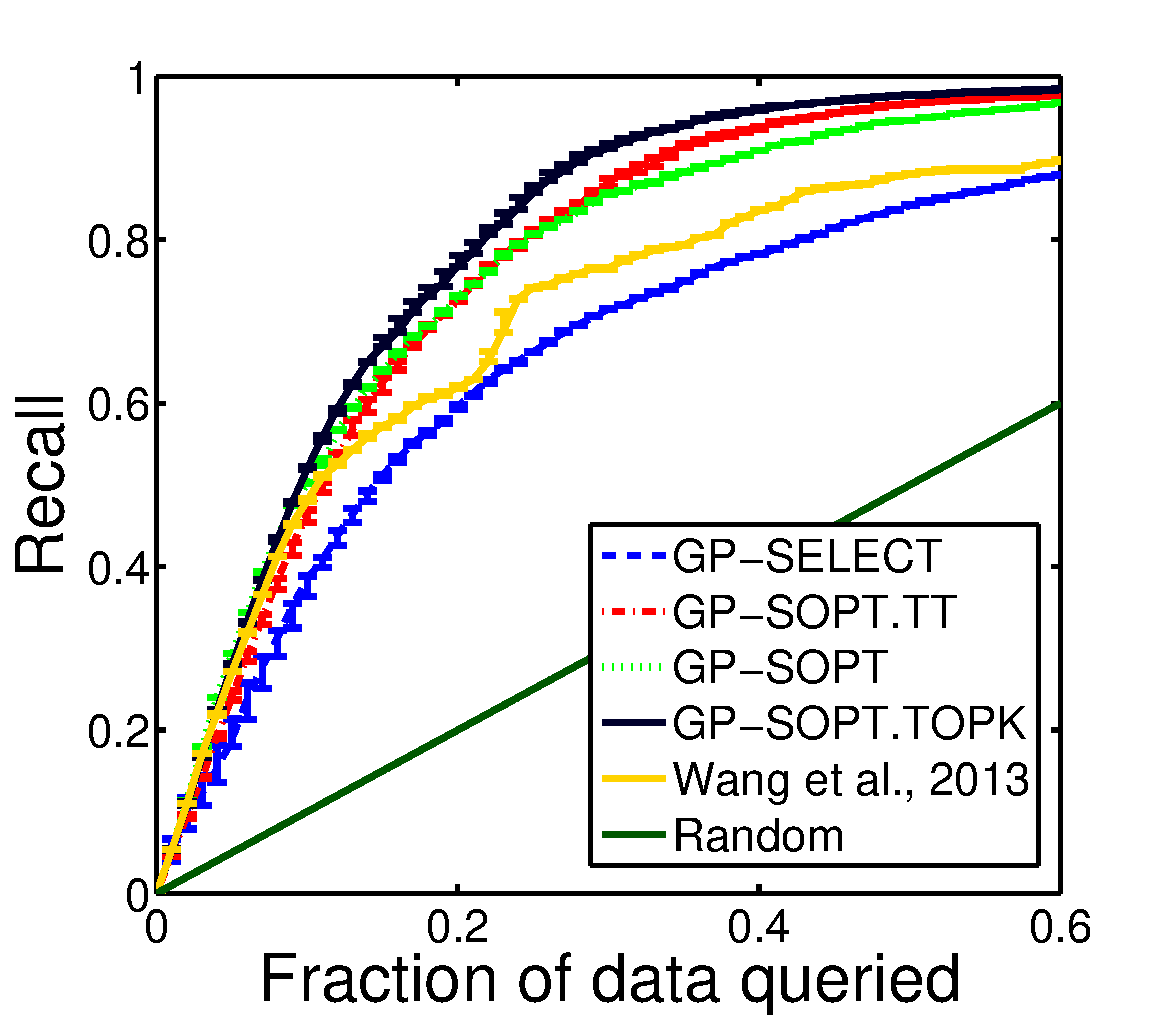
\includegraphics[width=0.5\linewidth, height=0.4\linewidth]{populated_places_5000_result_5seeds_top15p_omega0-001_lapnorm0.pdf} & 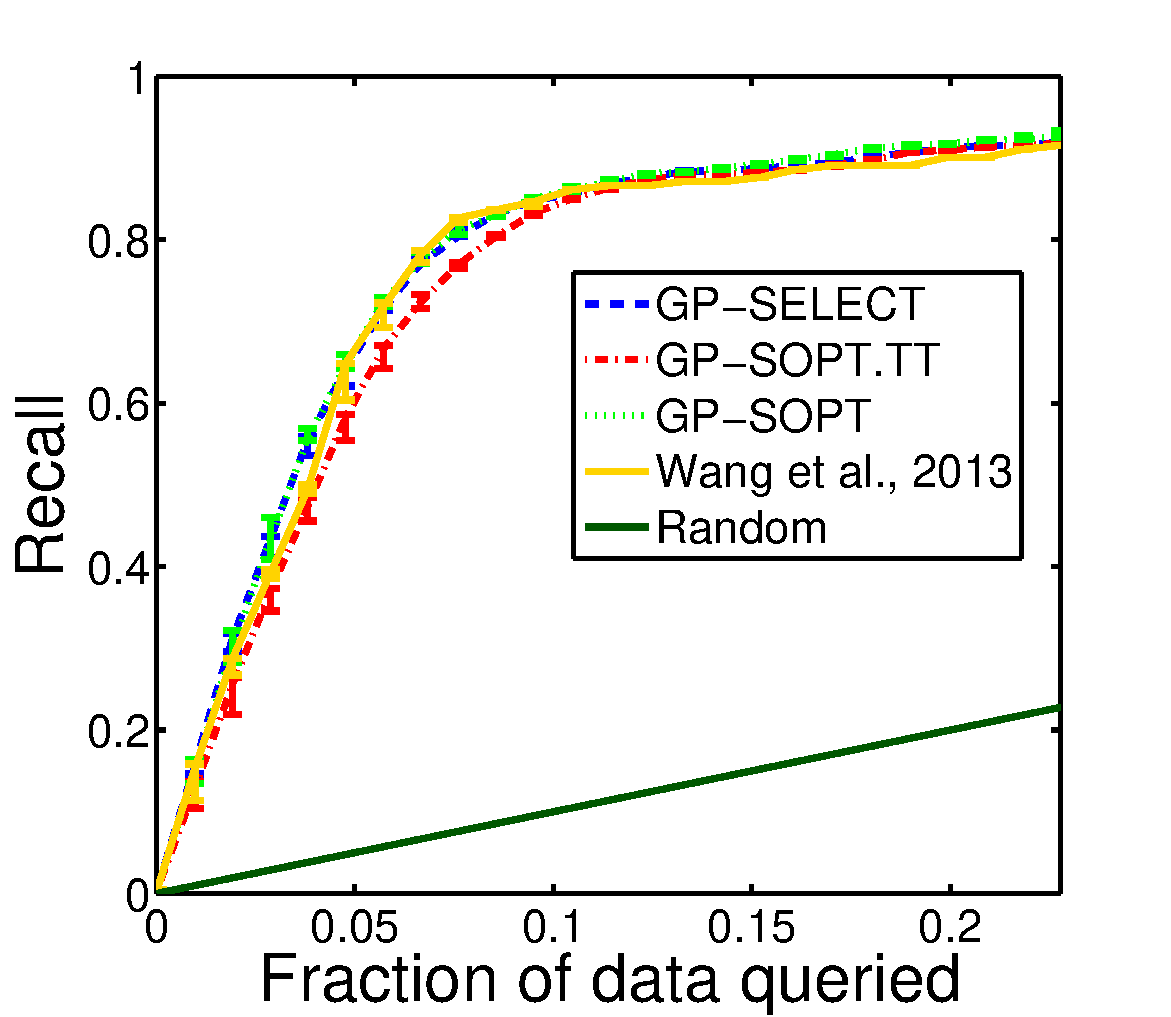
\includegraphics[width=0.5\linewidth, height=0.4\linewidth]{wiki_result_5seeds_top15p_omega0-001_lapnorm0.pdf} \vspace{-.5cm}\\ 
 Populated places & Wiki pages \\ 
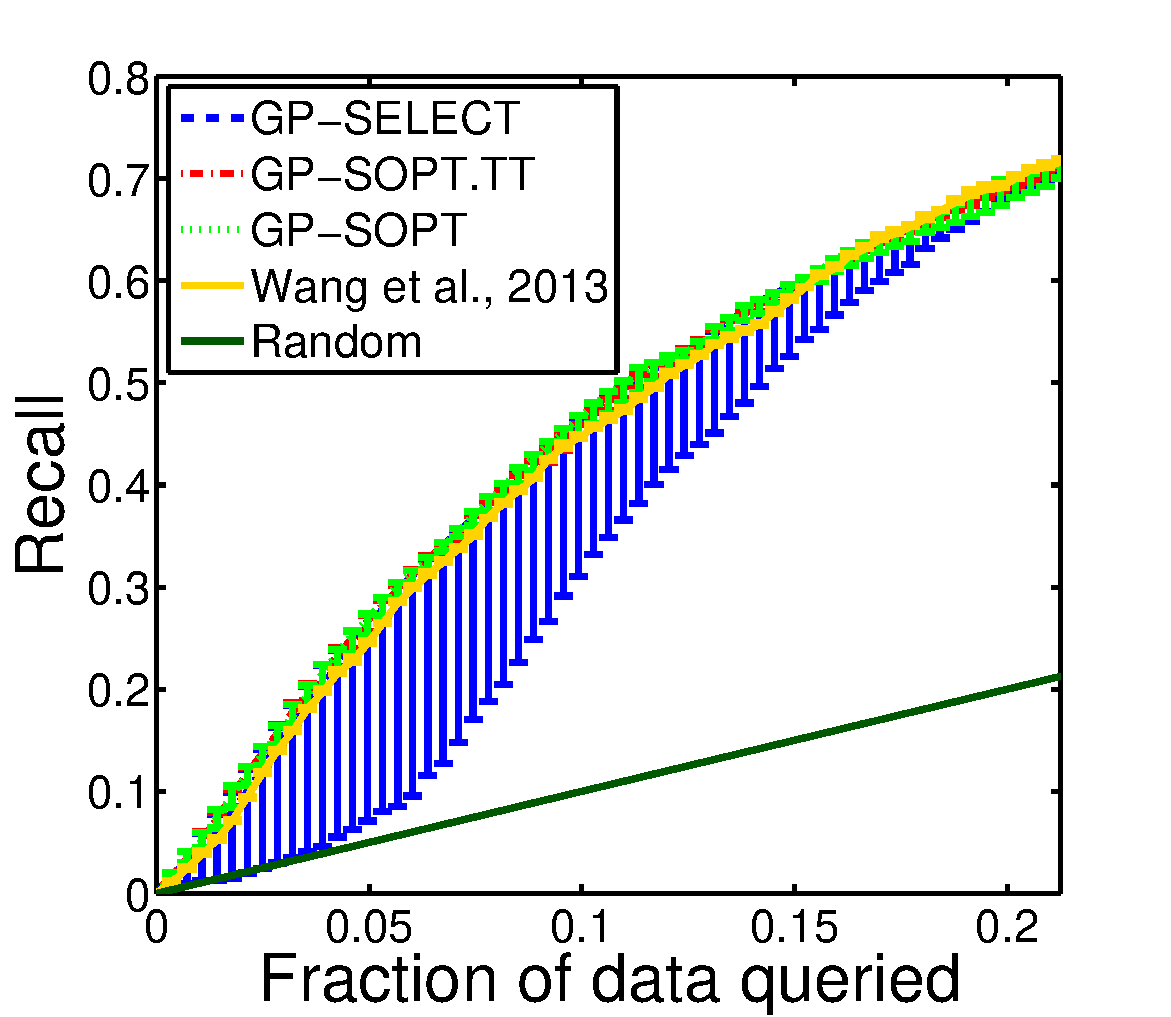
\includegraphics[width=0.5\linewidth, height=0.4\linewidth]{new_nips_result_5seeds_top15p_omega0-001_lapnorm0.pdf} & 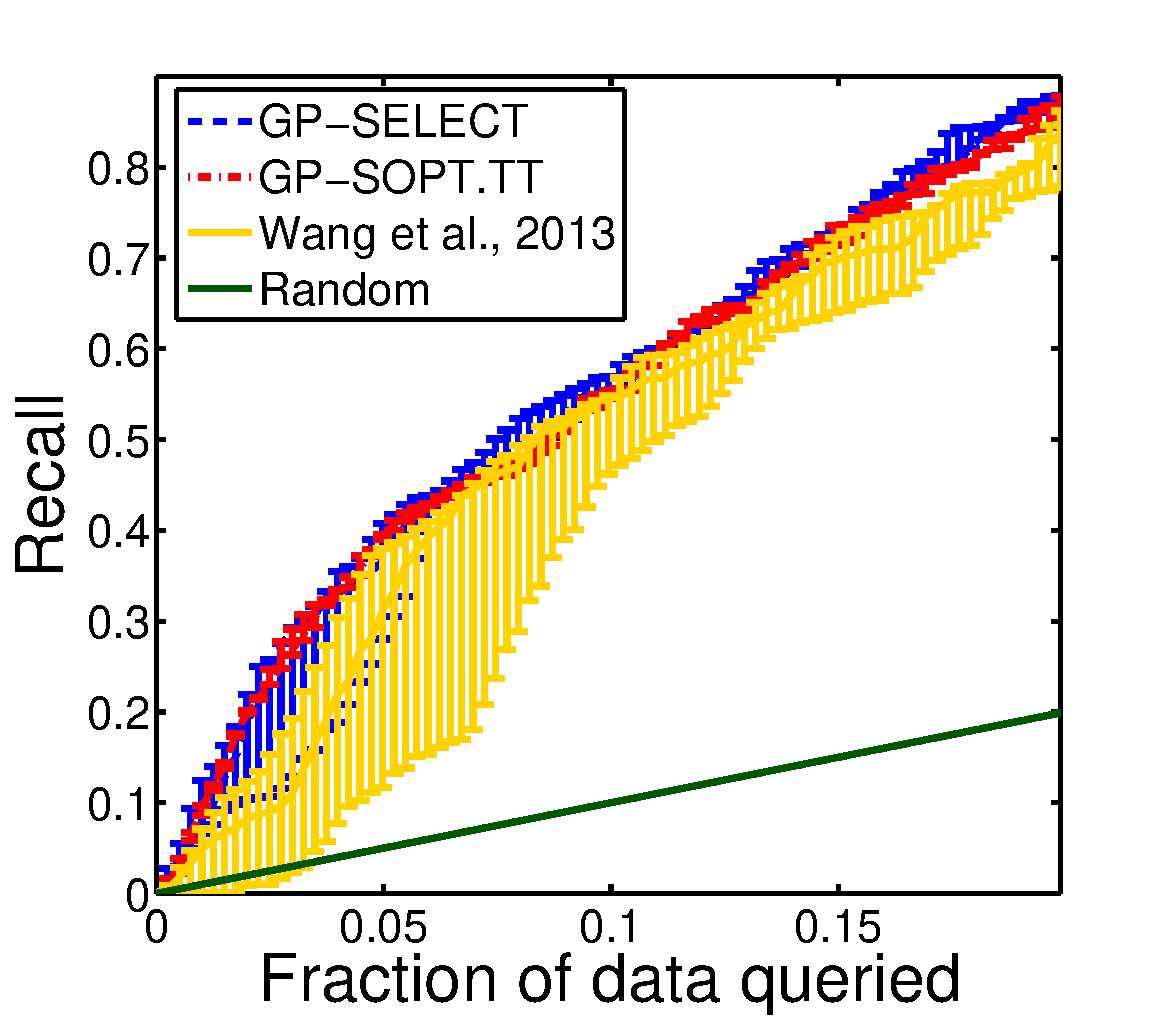
\includegraphics[width=0.5\linewidth, height=0.4\linewidth]{enron.pdf} \vspace{-.5cm}\\
Citation network & Enron e-mails
\end{tabular}
}
\vskip .5cm
\textcolor{red}{\textbf{Significant improvement over existing methods when exploration matters; more robust against outliers.}}\par
}
\vskip .5cm

% %%%%%%%%%%%%%%%%%%%%%%%%%%%%%%%%%%%%
% \paragraphHeader{Future Work}
% %%%%%%%%%%%%%%%%%%%%%%%%%%%%%%%%%%%%
% Spectral functions as exploration criteria; other graph kernels

% Active search on directed graphs; connect to matrix completion

% Allow new edges to emerge as a result of node query.

% \textbf{\normalsize Reference}
\hrule
{\normalsize
\begin{enumerate}
\setlength{\parskip}{0pt}
\setlength{\parsep}{0pt}
\setlength{\itemsep}{0pt}
% Peter Auer. Using confidence bounds for exploitation- exploration trade-offs. The Journal of Machine Learning Research, 3:397–422, 2003.
% Mikhail Belkin and Partha Niyogi. Laplacian eigenmaps and spectral techniques for embedding and clustering. In NIPS, volume 14, pages 585–591, 2001.
% Bernard Bercu, Abderrahmen Touati, et al. Exponential inequalities for self-normalized martingales with appli- cations. The Annals of Applied Probability, 18(5):1848– 1869, 2008.
% Michael W. Berry and Murray Browne. The 2001 annotated (by topic) Enron email data set. URL http://cis.jhu.edu/ ̃parky/Enron/Anno_ Topic_exp_LDC.pdf.
% Se ́bastien Bubeck, Gilles Stoltz, Csaba Szepesva ́ri, and Re ́mi Munos. Online optimization in X-armed bandits. In Advances in Neural Information Processing Systems, pages 201–208, 2009.
\item
Emile Contal, Vianney Perchet, and Nicolas Vayatis. \textbf{ GP-MI.} ICML 2014. %Gaussian process optimization with mutual information. In 31th International Conference on Machine Learning, 2014.
% Dennis D Cox and Susan John. Sdo: A statistical method for global optimization. Multidisciplinary design opti- mization: state of the art, pages 315–329, 1997.
% Varsha Dani, Thomas P Hayes, and Sham M Kakade. Stochastic linear optimization under bandit feedback. In COLT, pages 355–366, 2008.
% Roman Garnett, Yamuna Krishnamurthy, Xuehan Xiong, Jeff Schneider, and Richard Mann. Bayesian optimal ac- tive search and surveying. In ICML, 2012.
% Ming Ji and Jiawei Han. A variance minimization criterion to active learning on graphs. In AISTAT, 2012.
% Robert Kleinberg, Aleksandrs Slivkins, and Eli Upfal. Multi-armed bandits in metric spaces. In Proceedings of the fortieth annual ACM symposium on Theory of com- puting, pages 681–690. ACM, 2008.
\item
Andreas Krause, Ajit Singh, and Carlos Guestrin. \textbf{Sensor placement.} JMLR 2008.
% sensor placements in Gaussian processes: The- ory, efficient algorithms and empirical studies. Jour- nal of Machine Learning Research (JMLR), 9:235–284, February 2008.
\item
Yifei Ma, Roman Garnett, and Jeff Schneider. \textbf{$\Sigma$-optimality.} NIPS 2013. % in active learning on Gaussian random fields. In NIPS, 2013.
% Carey E. Priebe, John M. Conroy, David J. Marchette, and Youngser Park. Scan statistics on Enron graphs. URL http://cis.jhu.edu/ ̃parky/ Enron/enron.html.
% Carl Edward Rasmussen and Christopher KI Williams. Gaussian processes for machine learning, volume 1. MIT press Cambridge, MA, 2006.
% Herbert Robbins. Some aspects of the sequential design of experiments. In Herbert Robbins Selected Papers, pages 169–177. Springer, 1985.
% Burr Settles. Active learning literature survey. University of Wisconsin, Madison, 52(55-66):11, 2010.
\item
Niranjan Srinivas, Andreas Krause, Sham M Kakade, and Matthias Seeger. \textbf{GP-UCB.} TIT'12 %Information-theoretic regret bounds for gaussian process optimization in the bandit setting. In- formation Theory, IEEE Transactions on, 58(5):3250– 3265, 2012.
% Joshua B Tenenbaum, Vin De Silva, and John C Langford. A global geometric framework for nonlinear dimension- ality reduction. Science, 290(5500):2319–2323, 2000.
\item
Michal Valko, R{\'e}mi Munos, Branislav Kveton, Tom{\'a}{\v{s}} Koc{\'a}k. \textbf{Spectral Bandits.} ICML'14
% Spectralbanditsforsmoothgraphfunctions. In 31th International Conference on Machine Learning, 2014.
% Hastagiri P Vanchinathan, Andreas Marfurt, Charles- Antoine Robelin, Donald Kossmann, and Andreas Krause. Adaptively selecting valuable diverse sets via Gaussian processes and submodularity. In NIPS Work- shop on Discrete and Combinatorial Problems in Ma- chine Learning (DISCML) 2013: Theory and Applica- tions, 2013.
\item
Xuezhi Wang, Roman Garnett, and Jeff Schneider. \textbf{Active search on graphs.} SIGKDD 2013.
\item
Xiaojin Zhu, Zoubin Ghahramani, John Lafferty, et al.  \textbf{Semi-supervised GRF.} ICML 2003.
% Semi-supervised learning using gaussian fields and har- monic functions. In ICML, volume 3, pages 912–919, 2003a.
% \item
% Xiaojin Zhu, John Lafferty, and Zoubin Ghahramani. Com- bining active learning and semi-supervised learning us- ing gaussian fields and harmonic functions. In ICML 2003 workshop on the continuum from labeled to unla- beled data in machine learning and data mining, pages 58–65, 2003b.
\end{enumerate}
}

% \paragraphHeader{References}
\end{multicols}
\end{document}
